% !TEX encoding = UTF-8 Unicode
\documentclass{article}

\usepackage{multirow}
\usepackage[bottom]{footmisc}
\usepackage{url}
\usepackage{hyperref}
\usepackage{xepersian}
\usepackage{ulem}
\usepackage{enumitem}


\settextfont{XB Zar}

\renewcommand{\footnoterule}{
	\hrule width 3in
}
\rightfootnoterule

\title{\textbf{گام اول پروژه درس تحلیل و طراحی سیستم‌ها}}

\author{سید پارسا میرطاهری - ۹۵۱۰۹۳۹۴ \\ کیارش گل‌زردی - ۹۵۱۰۵۸۵۱}

\begin{document}

\date{}

\maketitle

\section{سند موارد کاربرد}

\subsection{نمودار موارد کاربرد}

\begin{figure}[htp]
\includegraphics[width = 1\textwidth]{../Use case Diagram/Use case Diagram.png}
\caption{\lr{Use Case Diagram}}
\label{usecase}
\end{figure}


\subsection{توصیف موارد کاربرد}

\begin{center}
\bgroup
\def\arraystretch{1.5}
\begin{tabular} {|p{0.23\textwidth}|p{0.7\textwidth}|}
\hline
 مورد کاربرد & 
 به مزایده گذاشتن کالا
\\ \hline
 شناسه &
۱
\\ \hline
توضیح مختصر &
کاربر مشخصات کالای خود را وارد می‌کند و با تعیین یک قیمت پایه آن را به مزایده می‌گذارد.
پس از تایید تیم بازبینی مزایده روی سایت قرار می‌گیرد.
\\ \hline
کنش‌گر(های) اولیه &
کاربر
\\ \hline
کنش‌گر(های) ثانویه &
ندارد
\\ \hline
پیش‌نیازها &
کاربر وارد سیستم شده است.
\\ \hline
روند اصلی &
\begin{enumerate}[nosep,topsep=0cm]
\item
کاربر مشخصات کالای خود را وارد می‌کند.
\item
کاربر برای کالای خود قیمت پایه تعیین می‌کند.
\item
کاربر درخواست ثبت آگهی مزایده را ارسال می‌کند.
\item
آگهی برای بررسی در اختیار تیم بازبینی قرار می‌گیرد.
\end{enumerate}
\\ \hline
پس‌نیازها &
آگهی برای بررسی تیم بازبینی در سیستم ثبت می‌شود.
\\ \hline
روند جایگزین &
در صورت لغو فرایند ثبت آگهی توسط کاربر فرم درخواست بسته می‌شود و اطلاعاتی ثبت نمی‌شود.
\\ \hline
\end{tabular}
\egroup
\end{center}

\newpage

\begin{center}
\bgroup
\def\arraystretch{1.5}
\begin{tabular} {|p{0.23\textwidth}|p{0.7\textwidth}|}
\hline
 مورد کاربرد & 
طرح پیشنهاد بالاتر
\\ \hline
 شناسه &
۲
\\ \hline
توضیح مختصر &
کاربر برای خرید کالایی که مزایدهٔ آن در جریان است یک پیشنهاد با ارزش بیشتر مساوی حداقل پیشنهاد فعلی لازم برای کالا ارائه می‌دهد.
\\ \hline
کنش‌گر(های) اولیه &
کاربر
\\ \hline
کنش‌گر(های) ثانویه &
ندارد
\\ \hline
پیش‌نیازها &
کاربر وارد سیستم شده است و مزایدهٔ کالا در جریان است.
\\ \hline
روند اصلی &
\begin{enumerate}[nosep,topsep=0cm]
\item
کاربر میزان ارزش پیشنهادی خود را برای خرید کالا اعلام می‌کند.
\item
در صورتی که میزان پیشنهادی از کف لازم بیشتر باشد و کاربر نیز به آن میزان در حسابش اعتبار داشته باشد پیشنهاد ثبت می‌شود.
\item
به میزان ارزش پیشنهادی از اعتبار کاربر کم می‌شود و در وضعیت رزرو قرار می‌گیرد و اعتبار رزرو شدهٔ آخرین پیشنهاد دهنده از حالت رزرو خارج می‌شود.
\item
وضعیت آخرین پیشنهاد مزایده به روز رسانی می‌شود.
\item
به روز رسانی وضعیت مزایده به اطلاع مزایده گذارنده و آخرین نفر پیشنهاد دهنده می‌رسد.
\end{enumerate}
\\ \hline
پس‌نیازها &
در صورت ثبت شدن پیشنهاد وضعیت آخرین پیشنهاد به روز رسانی شده و اعتبار پیشنهاد دهندهٔ آخر پس داده شده و از اعتبار پیشنهاد دهندهٔ فعلی کاسته می‌شود.
\\ \hline
روند جایگزین &
در صورتی که کاربر فرایند پیشنهاد را متوقف کند و یا پیشنهادش کافی نباشد و یا بیش از اعتبارش باشد وضعیت مزایده تغییری نمی‌کند.
\\ \hline
\end{tabular}
\egroup
\end{center}

\newpage

\begin{center}
\bgroup
\def\arraystretch{1.5}
\begin{tabular} {|p{0.23\textwidth}|p{0.7\textwidth}|}
\hline
 مورد کاربرد & 
نهایی شدن مزایده
\\ \hline
 شناسه &
۳
\\ \hline
توضیح مختصر &
با پایان زمان مزایده اگر خریداری پیدا شده باشد تراکنش خرید برای فروشنده و خریدار ثبت شده و امکان تایید تحویل برای خریدار فعال می‌شود.
\\ \hline
کنش‌گر(های) اولیه &
زمان
\\ \hline
کنش‌گر(های) ثانویه &
ندارد
\\ \hline
پیش‌نیازها &
زمان مزایده در این لحظه به پایان رسده باشد.
\\ \hline
روند اصلی &
\begin{enumerate}[nosep,topsep=0cm]
\item
زمان مزایده به پایان می‌رسد.
\item
وضعیت مزایده به روز رسانی می‌شود و آخرین پیشنهاد دهنده به عنوان خریدار معرفی می‌شود.
\item
ثبت خرید به اطلاع خریدار و فروشنده می‌رسد و اطلاعات تماس طرفین به یکدیگر منتقل می‌شود.
\item
امکان تایید تحویل برای خریدار فعال می‌شود.
\item
روز شمار نهایی کردن خرید آغاز می‌شود.
\end{enumerate}
\\ \hline
پس‌نیازها &
وضعیت مزایده نهایی شده است و گزینهٔ تایید تحویل برای خریدار فعال شده است.
\\ \hline
روند جایگزین &
در صورتی که خریدار برای کالا پیدا نشده باشد تنها وضعیت مزایده نهایی می‌شود و اتفاق دیگری صورت نمی‌پذیرد.
\\ \hline
\end{tabular}
\egroup
\end{center}

\newpage

\begin{center}
\bgroup
\def\arraystretch{1.5}
\begin{tabular} {|p{0.23\textwidth}|p{0.7\textwidth}|}
\hline
 مورد کاربرد & 
 تایید تحویل
\\ \hline
 شناسه &
۴
\\ \hline
توضیح مختصر &
خریدار پس از تحویل کالا از طریق فروشنده گزینهٔ تایید تحویل  را انتخاب می‌کند.
\\ \hline
کنش‌گر(های) اولیه &
کاربر
\\ \hline
کنش‌گر(های) ثانویه &
ندارد
\\ \hline
پیش‌نیازها &
زمان مزایدهٔ کالا تمام شده و کاربر مورد نظر خریدار نهایی کالاست و گزینهٔ تایید تحویل برای او فعال شده است. همچنین کاربر وارد سیستم شده است.
\\ \hline
روند اصلی &
\begin{enumerate}[nosep,topsep=0cm]
\item
کاربر گزینهٔ تایید تحویل را انتخاب می‌کند.
\item
اعتبار رزرو شدهٔ خریدار برای این کالا از اعتبار او کاسته می‌شود و اعتبار فروشنده به همین میزان با احتساب کارمزد سیستم افزایش می‌یابد.
\end{enumerate}
\\ \hline
پس‌نیازها &
اعتبار رزرو شدهٔ خریدار از اعتبار او کاسته می‌شود و اعتبار فروشنده افزایش می‌یابد. قسمتی از مبلغ نیز به حساب سیستم ریخته می‌شود.
\\ \hline
روند جایگزین &
ندارد.
\\ \hline
\end{tabular}
\egroup
\end{center}

\newpage

\begin{center}
\bgroup
\def\arraystretch{1.5}
\begin{tabular} {|p{0.23\textwidth}|p{0.7\textwidth}|}
\hline
 مورد کاربرد & 
افزایش اعتبار حساب کاربری
\\ \hline
 شناسه &
۵
\\ \hline
توضیح مختصر &
کاربر با پرداخت هزینه اعتبار حساب خود را افزایش می‌دهد.
\\ \hline
کنش‌گر(های) اولیه &
کاربر
\\ \hline
کنش‌گر(های) ثانویه &
ندارد
\\ \hline
پیش‌نیازها &
کاربر وارد سیستم شده است.
\\ \hline
روند اصلی &
\begin{enumerate}[nosep,topsep=0cm]
\item
کاربر گزینهٔ افزایش اعتبار را انتخاب می‌کند.
\item
کاربر مبلغ مورد نظر برای افزایش اعتبار را بین یکی از چند گزینهٔ موجود و یا به صورت دلخواه وارد می‌کند.
\item
کاربر به درگاه بانکی متصل می‌شود.
\item
با تایید درگاه کاربر به سایت اصلی بازگردانده شده و اعتبار حساب او افزایش می‌یابد.
\end{enumerate}
\\ \hline
پس‌نیازها &
اعتبار حساب کاربر به میزان انتخاب شده افزایش می‌یابد.
\\ \hline
روند جایگزین &
در صورت انصراف کاربر از ادامهٔ کار، اعتبار حساب او تغییر نخواهد کرد.
\\ \hline
\end{tabular}
\egroup
\end{center}

\newpage

\section{نمودارهای فعالیت}

\begin{figure}[htp]
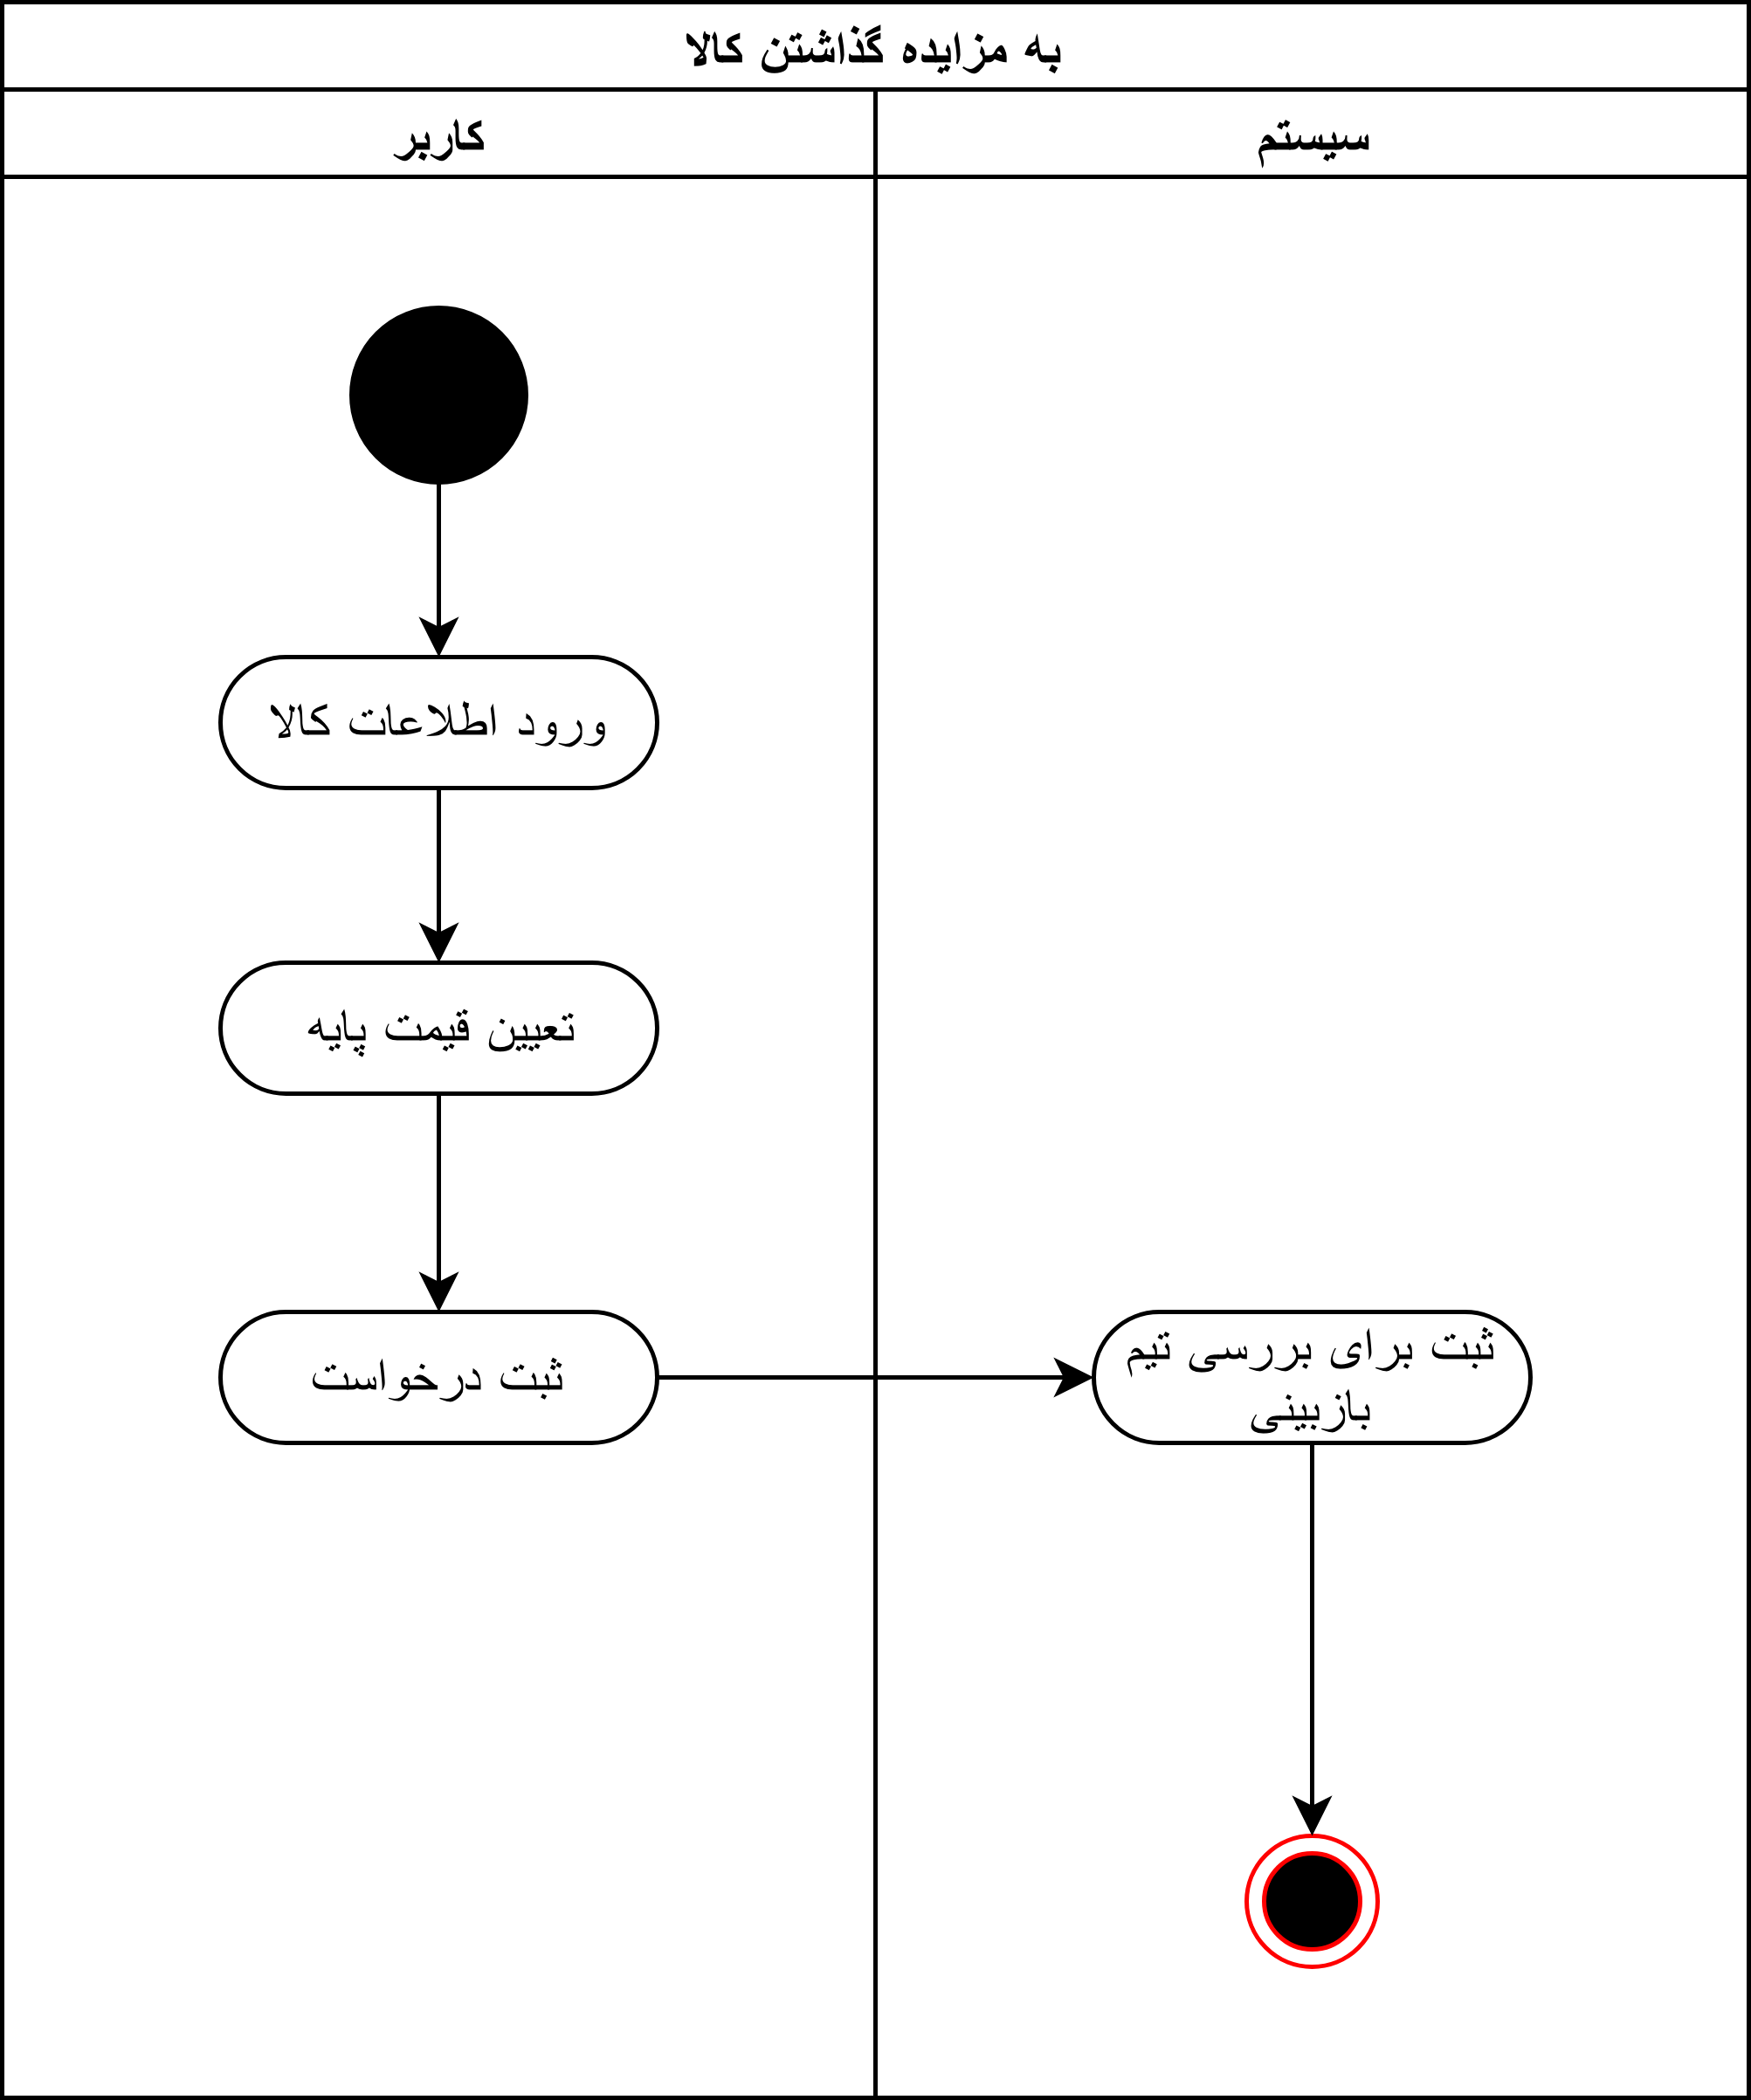
\includegraphics[width = 1\textwidth]{../Activity Diagrams/Activity 1.png}
\caption{\lr{Create an auction}}
\label{activity1}
\end{figure}

\begin{figure}[htp]
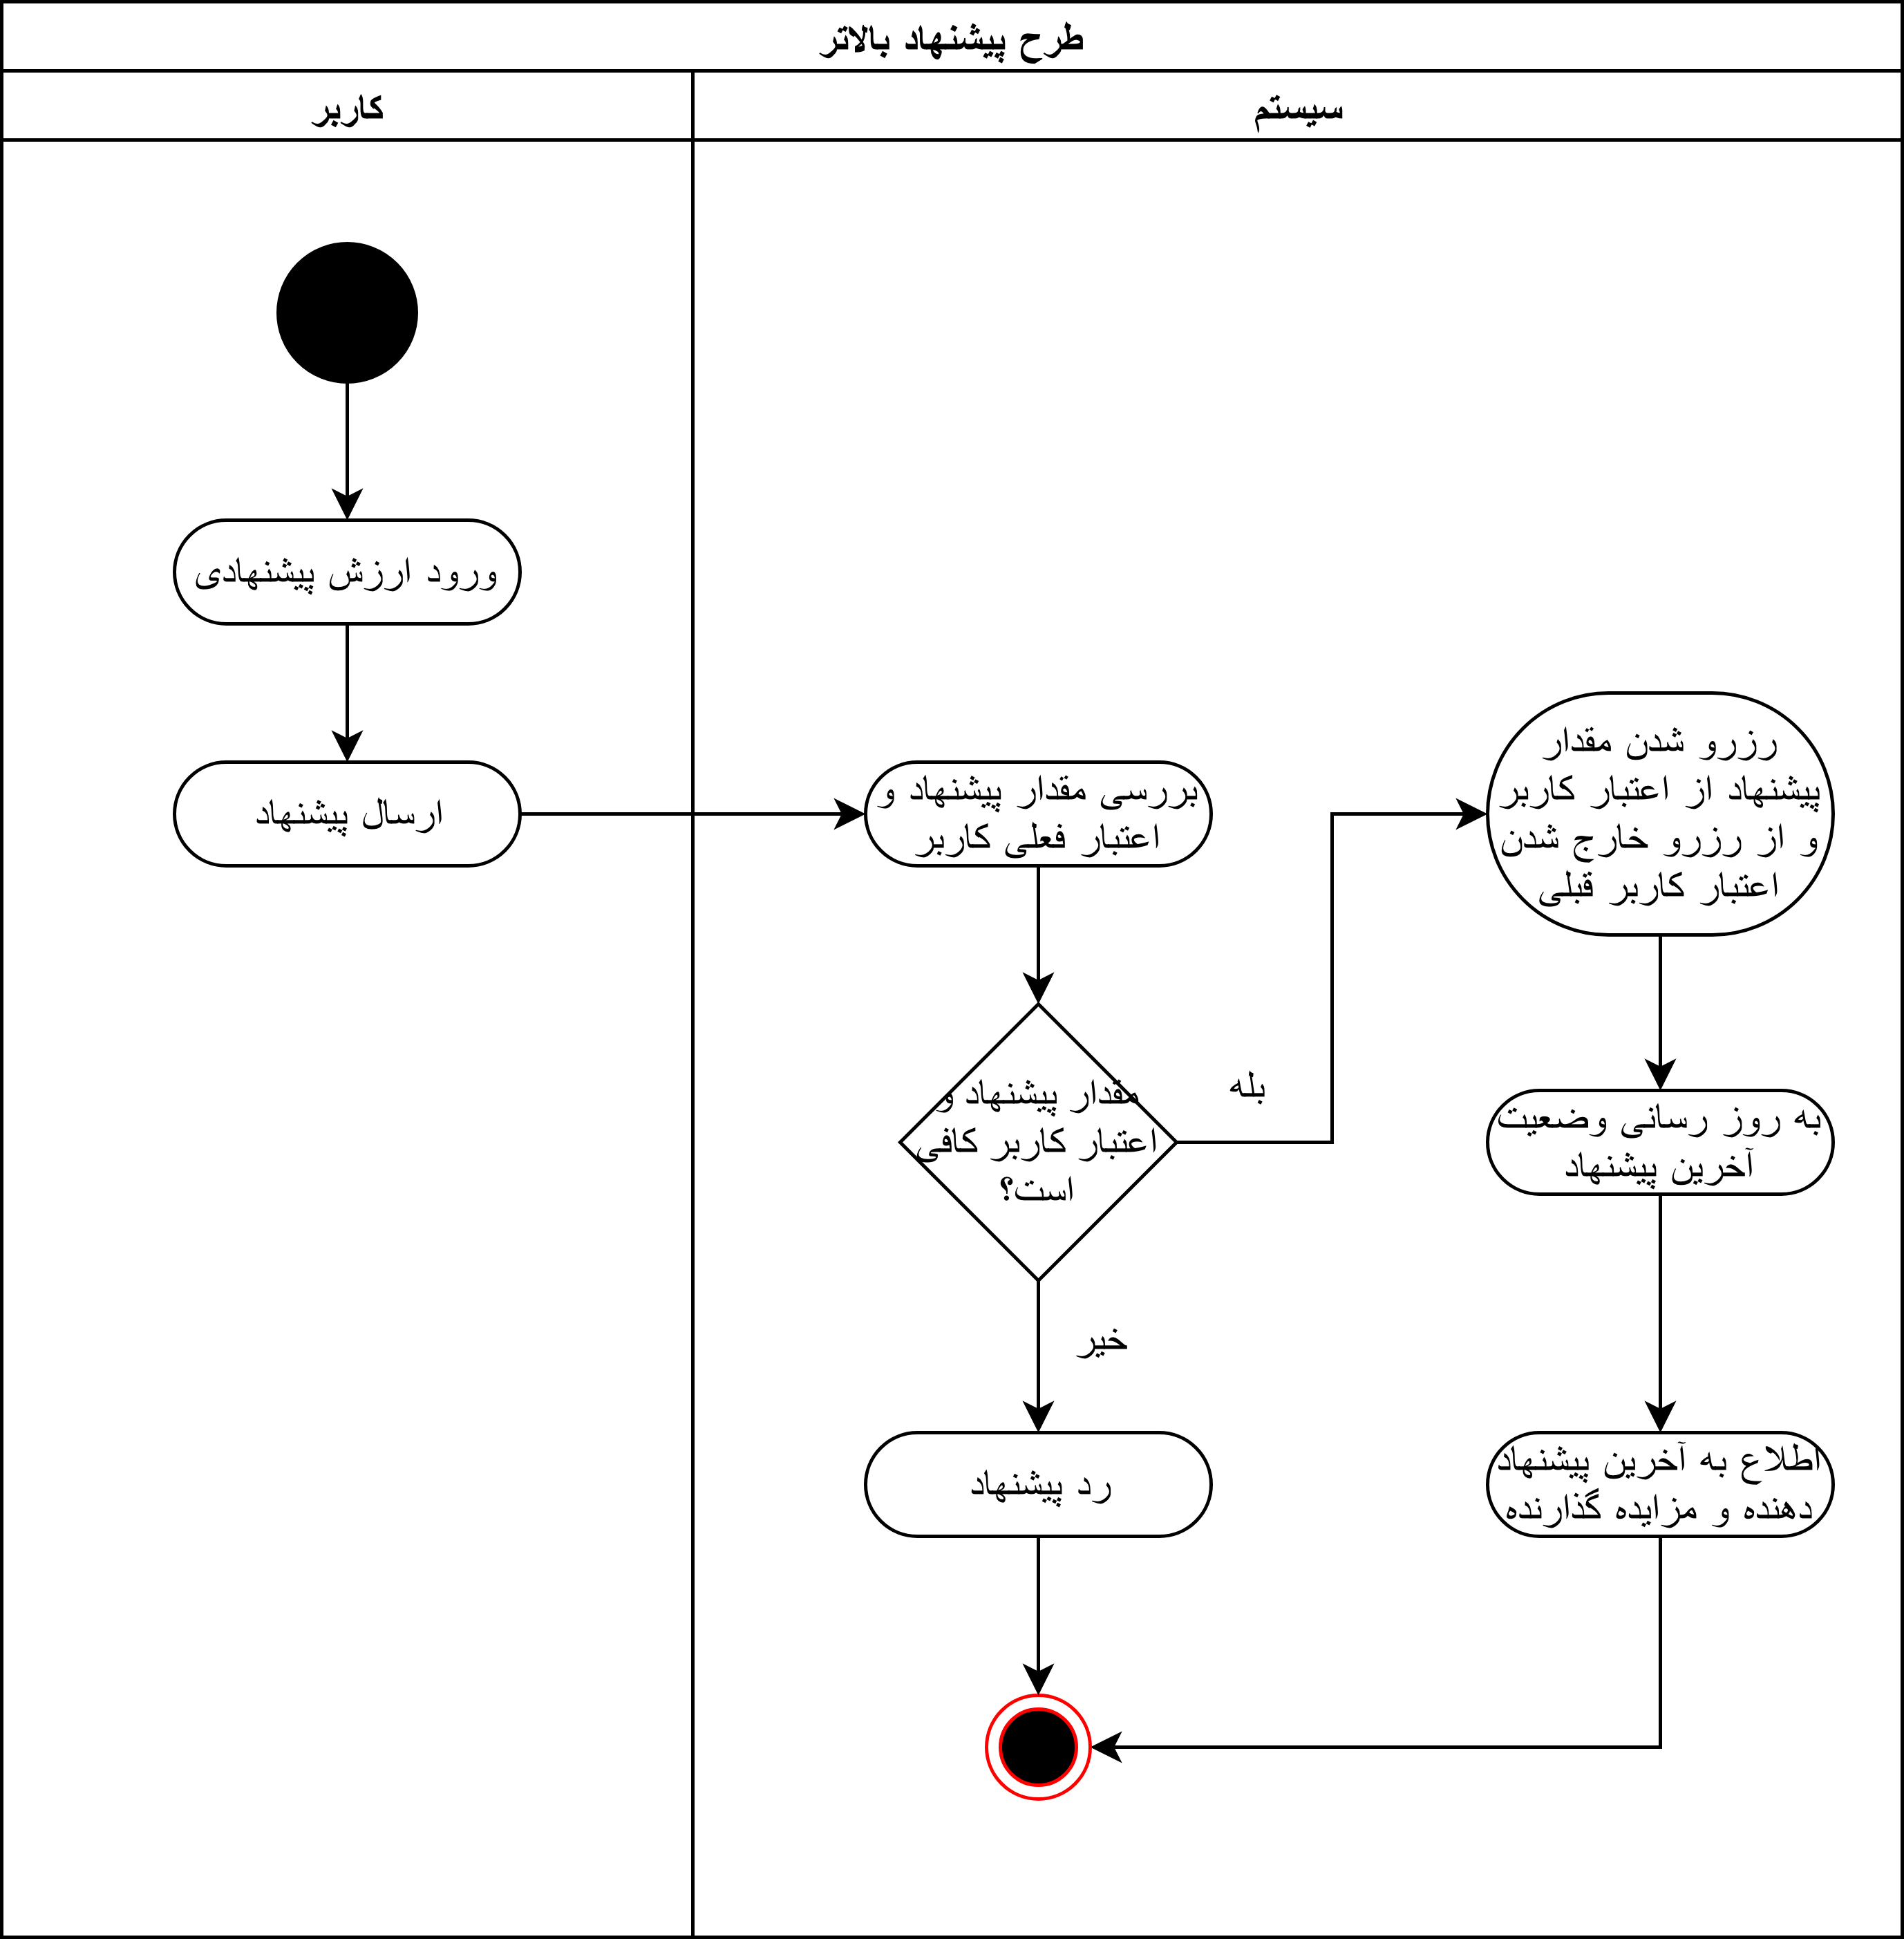
\includegraphics[width = 1\textwidth]{../Activity Diagrams/Activity 2.png}
\caption{\lr{Offer higher bid}}
\label{activity2}
\end{figure}

\begin{figure}[htp]
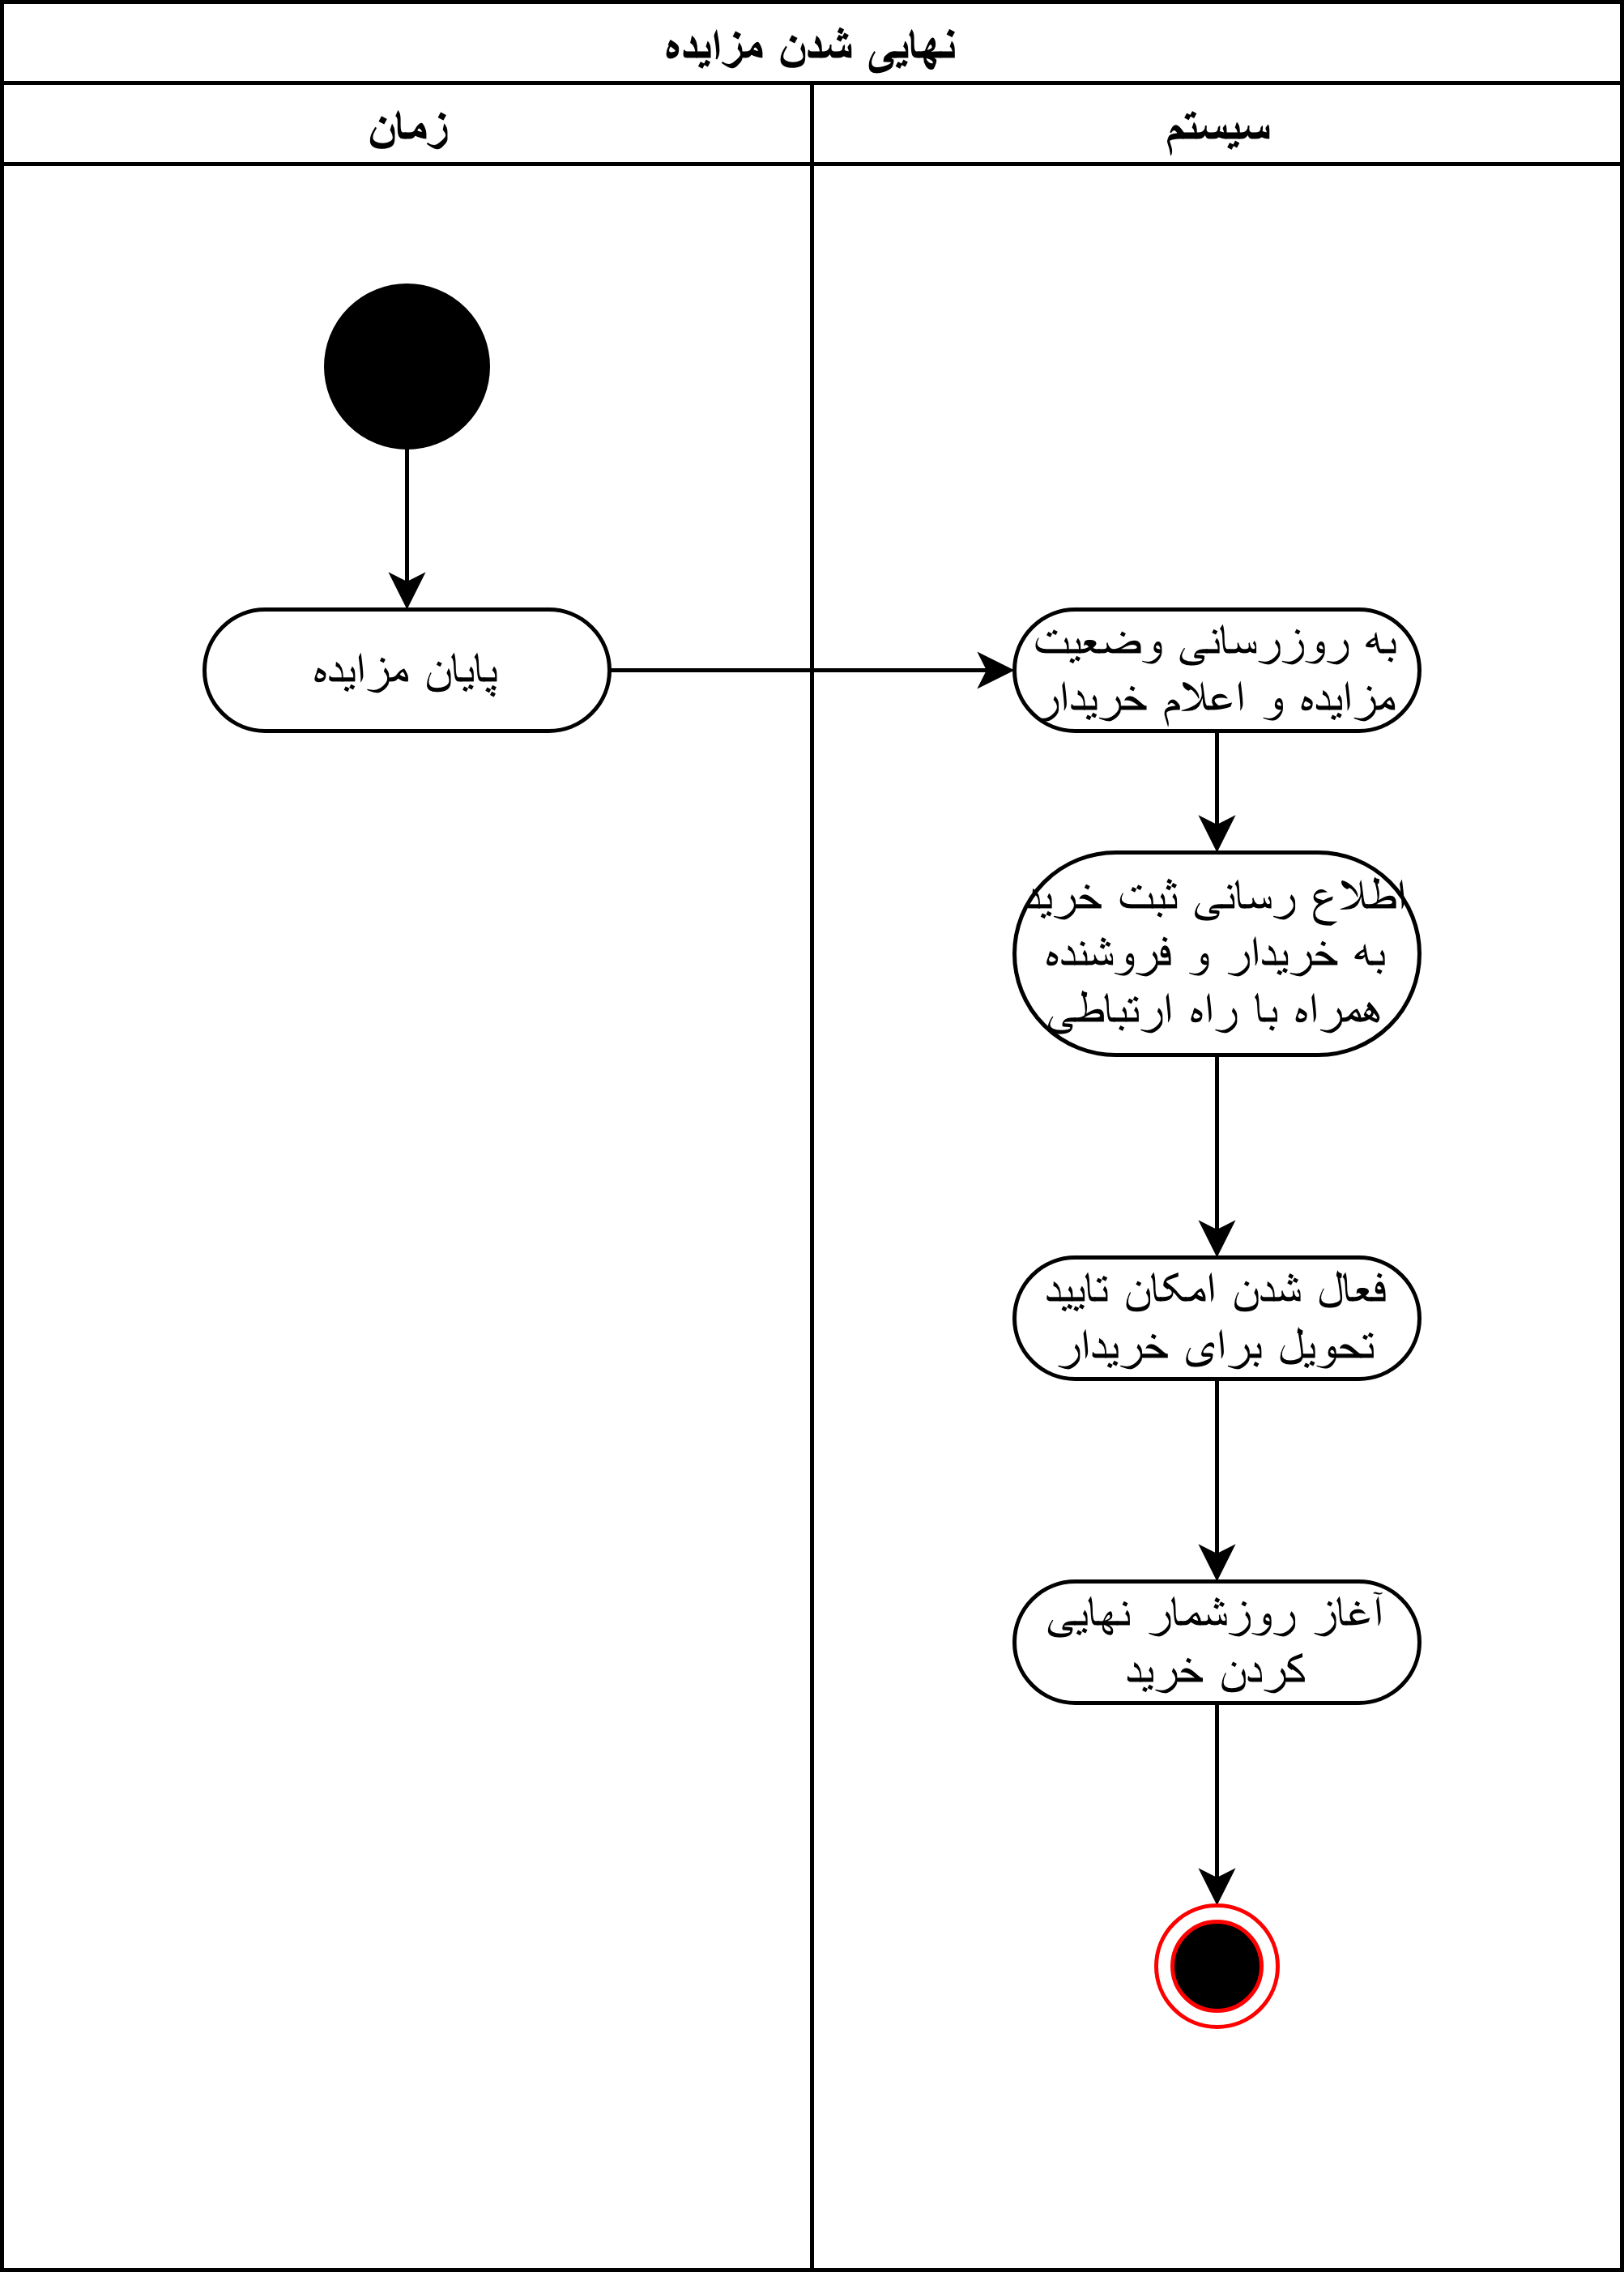
\includegraphics[width = 1\textwidth]{../Activity Diagrams/Activity 3.png}
\caption{\lr{Finalize an auction}}
\label{activity3}
\end{figure}

\begin{figure}[htp]
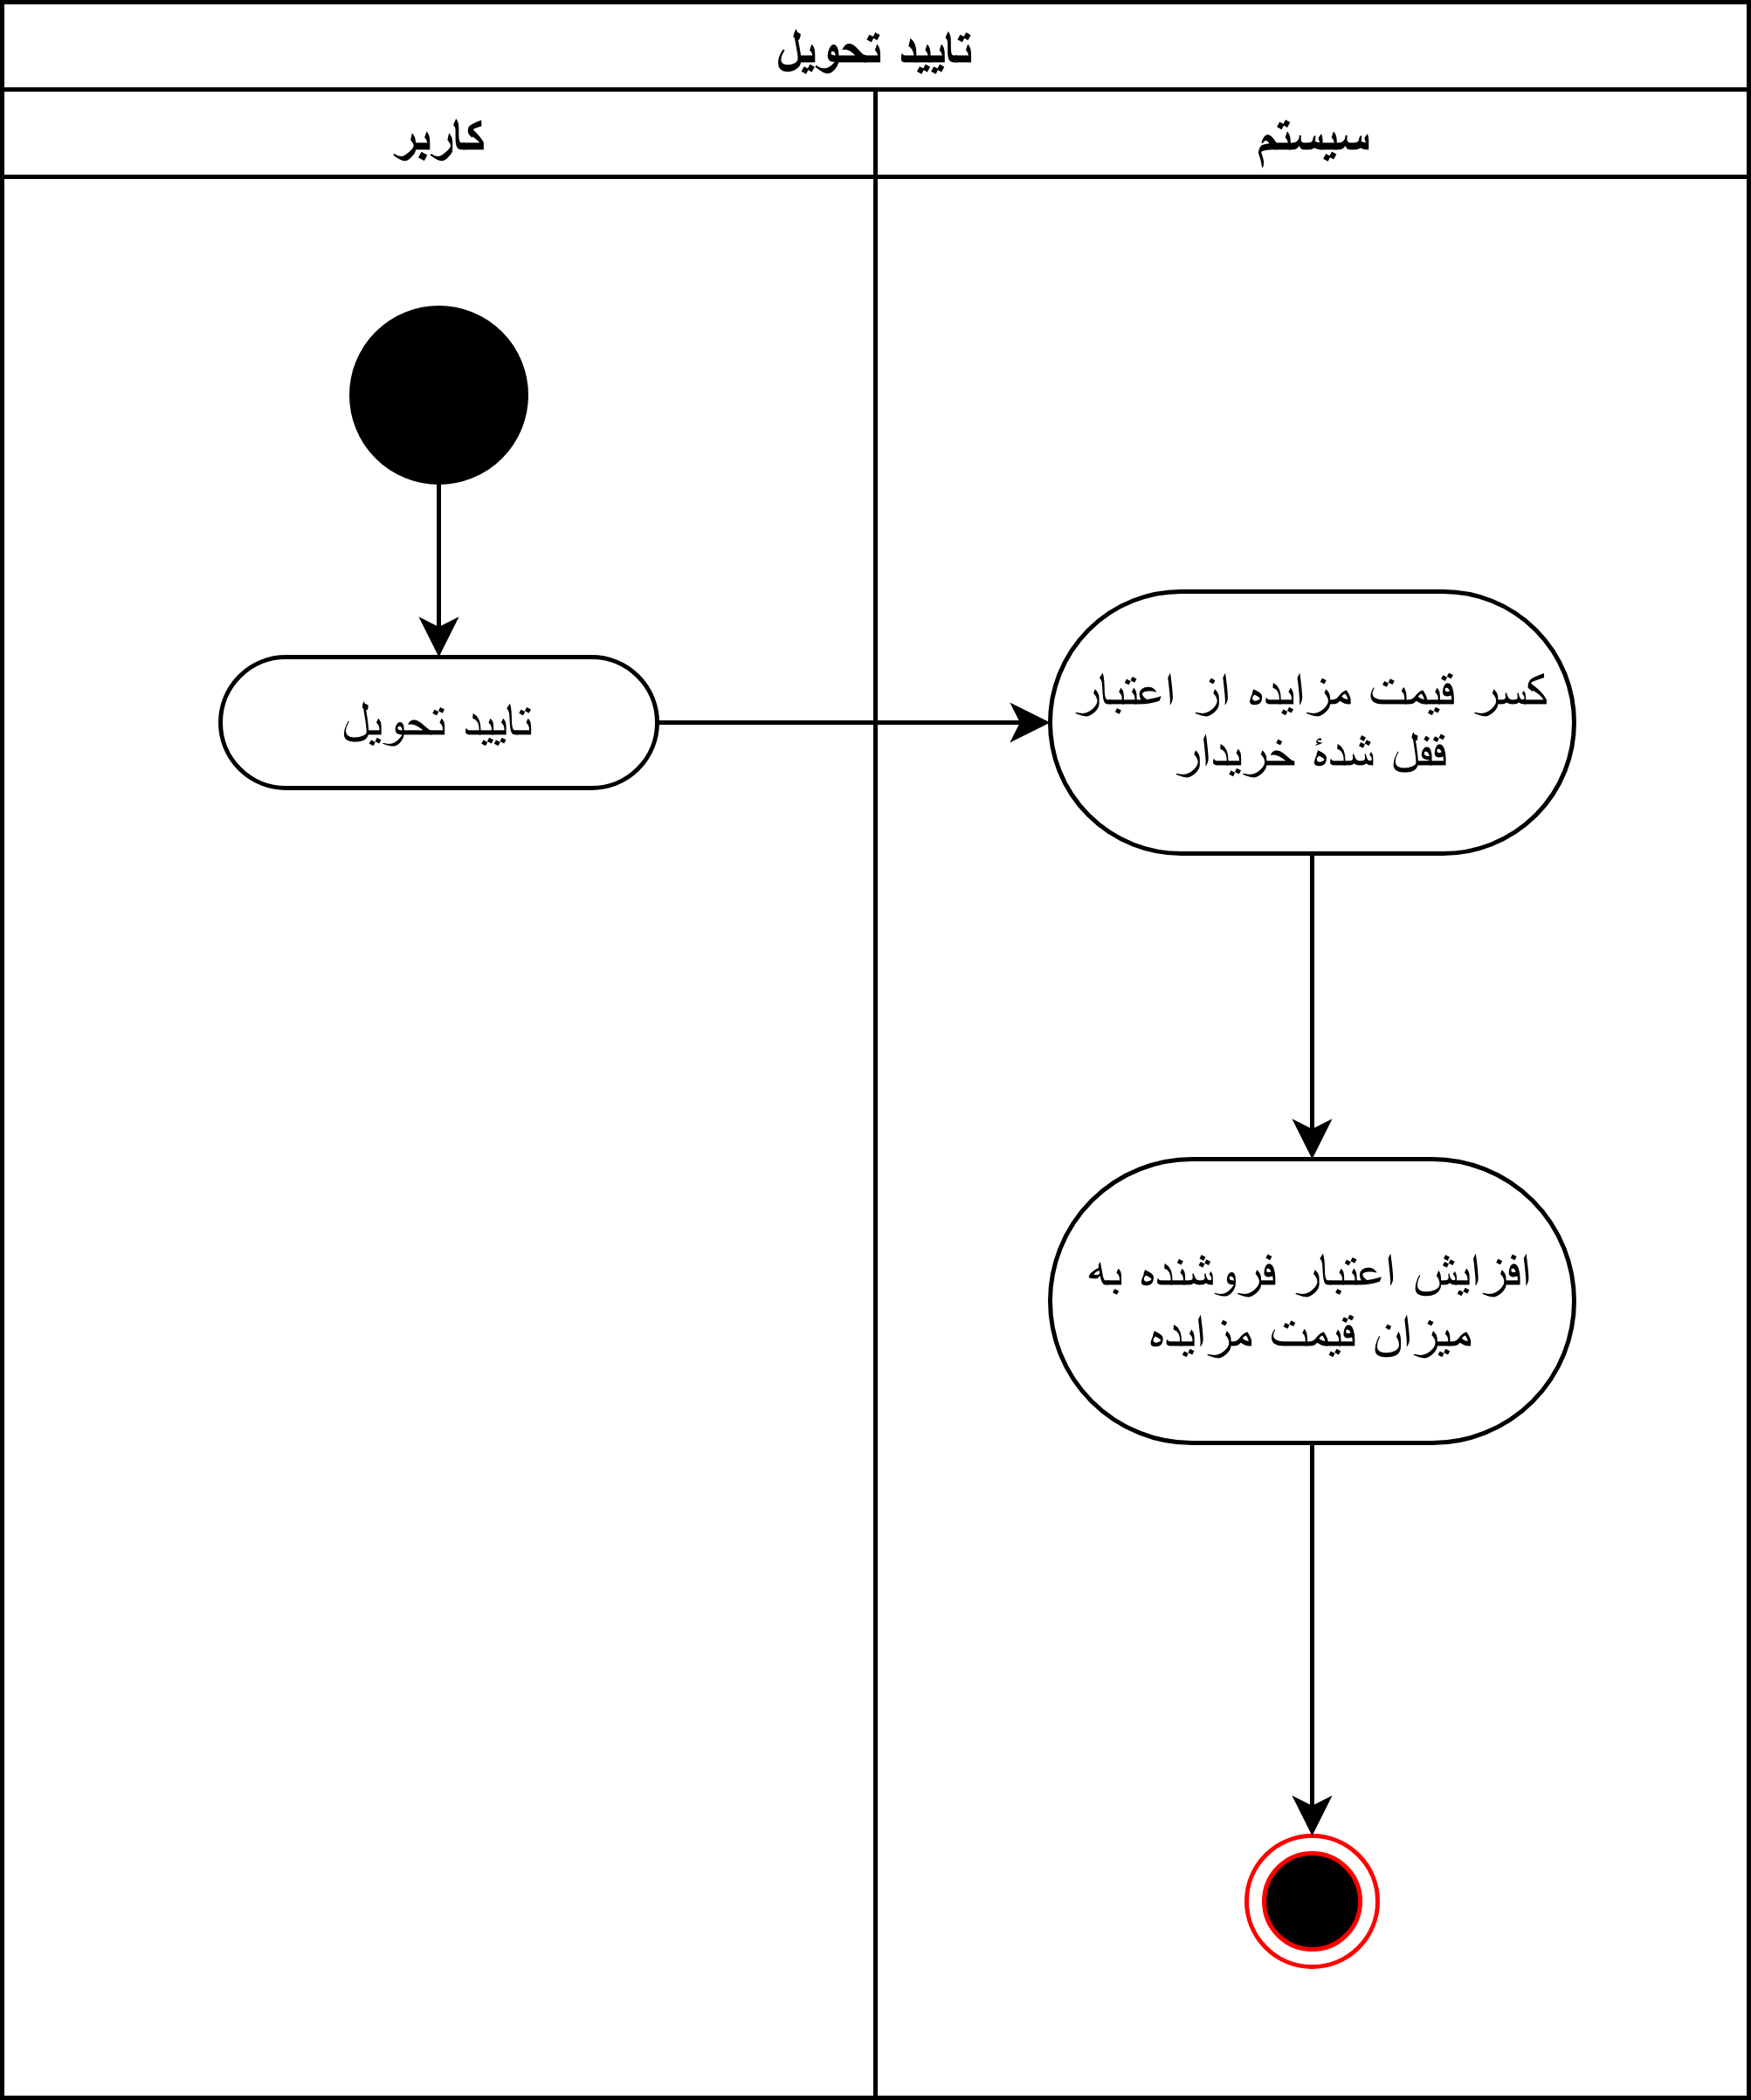
\includegraphics[width = 1\textwidth]{../Activity Diagrams/Activity 4.png}
\caption{\lr{Verify the delivery}}
\label{activity3}
\end{figure}

\begin{figure}[htp]
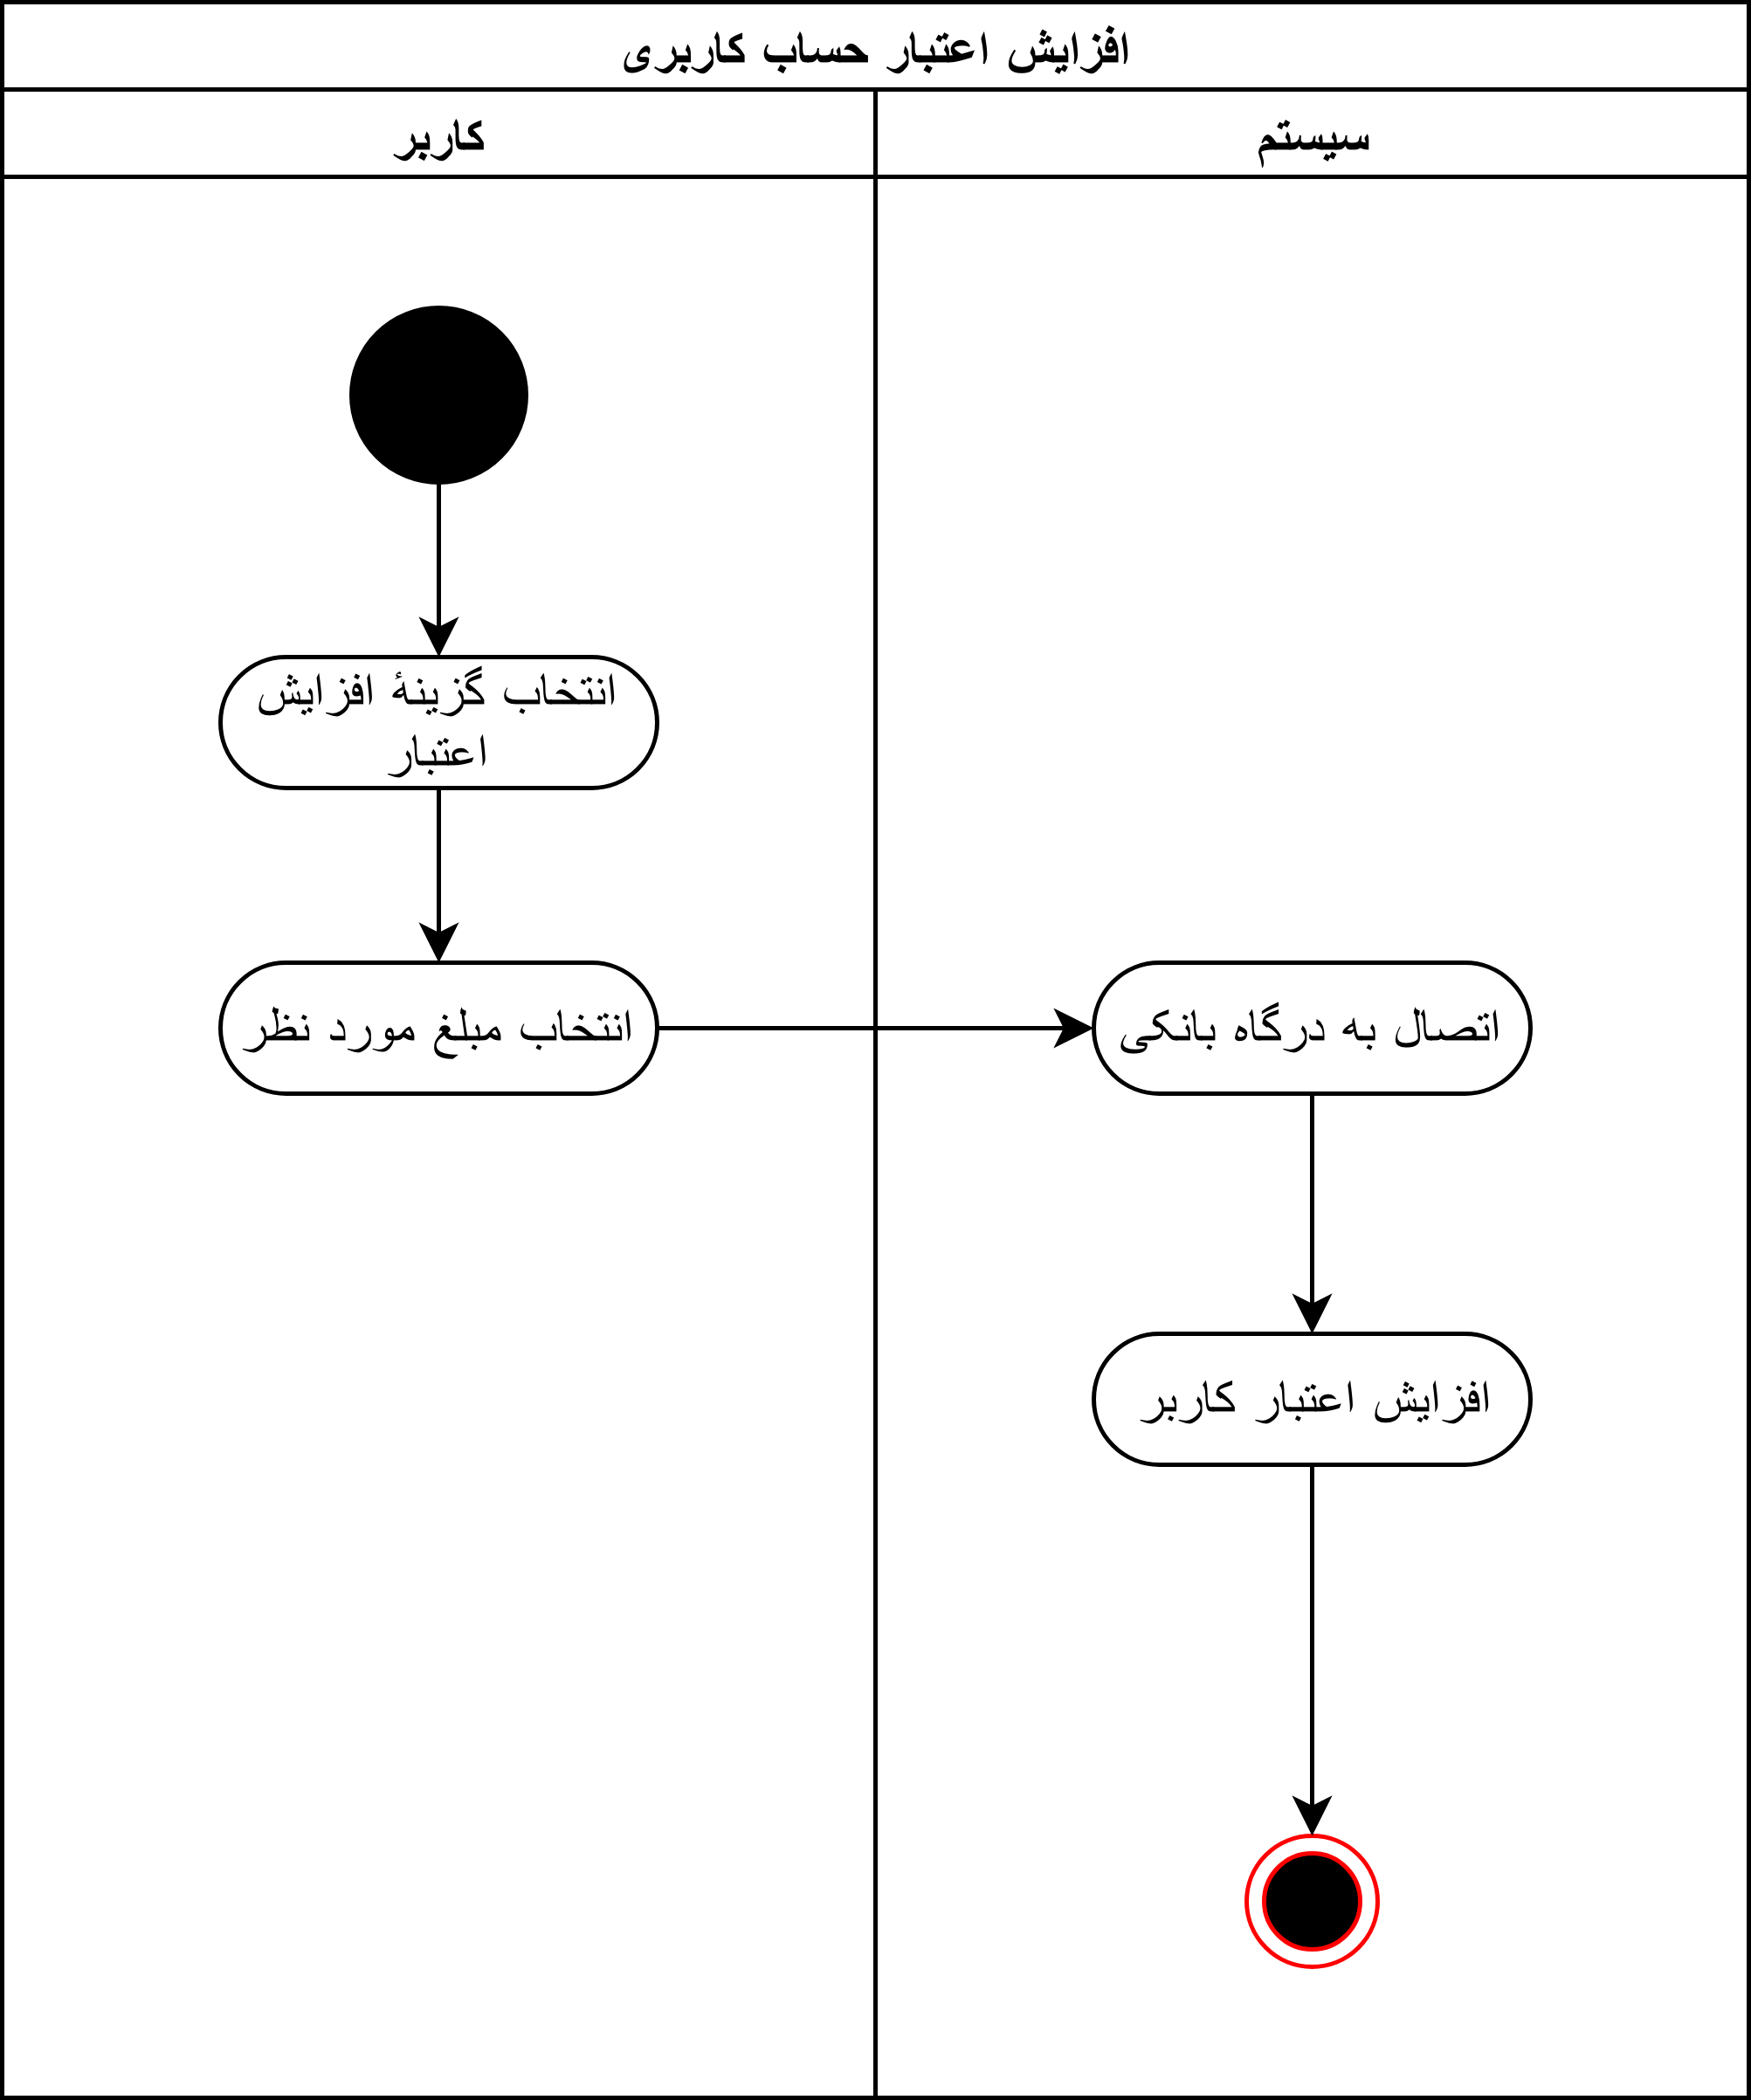
\includegraphics[width = 1\textwidth]{../Activity Diagrams/Activity 5.png}
\caption{\lr{Increase account credit}}
\label{activity4}
\end{figure}

\end{document}
